%
% File acl2017_supp.tex
%

\documentclass[11pt,a4paper]{article}
\usepackage{acl-onecolumn}
\usepackage{times}
\usepackage{url}
\usepackage{latexsym}
\usepackage{amsmath}
\usepackage{breqn}
\usepackage{pgfplotstable}
\usepackage{algorithm2e}
\usepackage{hhline}
\usepackage{multirow}
\usepackage[font=small]{caption}
\usepackage{subcaption}
\usepackage{color}
\usepackage{float}
\usepackage{lipsum,adjustbox}
\usepackage{tikz}
\usepackage{tikz-dependency}
\usepackage{enumitem}
\usepackage{xr}
\externaldocument{acl2017}
\usetikzlibrary{shapes,fit,calc,er,positioning,intersections,decorations.shapes,mindmap,trees}
\tikzset{decorate sep/.style 2 args={decorate,decoration={shape backgrounds,shape=circle,
      shape size=#1,shape sep=#2}}}
\newcommand{\oa}[1]{\footnote{\color{red} #1}}
\newcommand{\daniel}[1]{\footnote{\color{blue} #1}}
\newcommand{\com}[1]{}
\newcommand{\parser}[1]{TUPA\textsubscript{#1}}
\newcommand{\secref}[1]{Section~\ref{#1}}
\newcommand{\figref}[1]{Figure~\ref{#1}}
\newcommand{\tabref}[1]{Table~\ref{#1}}
\DeclareMathOperator*{\argmin}{argmin}
\DeclareMathOperator*{\argmax}{argmax}
\SetKwRepeat{Do}{do}{while}

\hyphenation{SemEval}
\hyphenation{PARSEVAL}
\hyphenation{DAGParser}
\hyphenation{TurboSemanticParser}
\hyphenation{MaltParser}

\title{Broad-Coverage Transition-Based UCCA Parsing \\ Supplementary Notes}

\begin{document}
\maketitle

\appendix
\section{Feature Templates}
\label{appendix:features}

\figref{fig:features} presents the feature templates used by \parser{Sparse}.
All feature templates define binary features.
The other classifiers use the same elements listed in the feature templates,
but all categorical features are replaced by vector embeddings,
and all count-based features are replaced by their numeric value.

For some of the features, we used the notion of \textit{head word},
defined by the $h^*$ function (see Appendix~\ref{appendix:conversion}).
While head words are not explicitly represented in the UCCA scheme, these
features prove useful as means of encoding word-to-word relations.

\begin{figure*}[h]
\centering
\begin{adjustbox}{margin=3pt,frame}
\begin{tabular}{l}
{\footnotesize Features from \cite{zhang2009transition}:} \\
\textbf{unigrams} \\
$s_0tde, s_0we, s_1tde, s_1we, s_2tde, s_2we, s_3tde, s_3we,$ \\
$b_0wtd, b_1wtd, b_2wtd, b_3wtd,$ \\
$s_0lwe, s_0rwe, s_0uwe, s_1lwe, s_1rwe, s_1uwe$ \\
\textbf{bigrams} \\
$s_0ws_1w, s_0ws_1e, s_0es_1w, s_0es_1e, s_0wb_0w, s_0wb_0td,$ \\
$s_0eb_0w, s_0eb_0td, s_1wb_0w, s_1wb_0td, s_1eb_0w, s_1eb_0td,$ \\
$b_0wb_1w, b_0wb_1td, b_0tdb_1w, b_0tdb_1td$ \\
\textbf{trigrams} \\
$s_0es_1es_2w, s_0es_1es_2e, s_0es_1eb_0w, s_0es_1eb_0td,$ \\
$s_0es_1wb_0w, s_0es_1wb_0td, s_0ws_1es_2e, s_0ws_1eb_0td$ \\
\textbf{separator} \\
$s_0wp, s_0wep, s_0wq, s_0wcq, s_0es_1ep, s_0es_1eq,$ \\
$s_1wp, s_1wep, s_1wq, s_1weq$ \\

\textbf{extended} \footnotesize \cite{zhu2013fast} \\
$s_0llwe, s_0lrwe, s_0luwe, s_0rlwe, s_0rrwe,$ \\
$s_0ruwe, s_0ulwe, s_0urwe, s_0uuwe, s_1llwe,$ \\
$s_1lrwe, s_1luwe, s_1rlwe, s_1rrwe, s_1ruwe$ \\
\end{tabular}
\begin{tabular}{l}
\textbf{disco} \footnotesize \cite{maier2015discontinuous} \\
$s_0xwe, s_1xwe, s_2xwe, s_3xwe,$ \\
$s_0xtde, s_1xtde, s_2xtde, s_3xtde,$ \\
$s_0xy, s_1xy, s_2xy, s_3xy$ \\
$s_0xs_1e, s_0xs_1w, s_0xs_1x, s_0ws_1x, s_0es_1x,$ \\
$s_0xs_2e, s_0xs_2w, s_0xs_2x, s_0ws_2x, s_0es_2x,$ \\
$s_0ys_1y, s_0ys_2y, s_0xb_0td, s_0xb_0w$ \\

{\footnotesize Features from \cite{tokgoz2015transition}:} \\
\textbf{counts} \\
$s_0P, s_0C, s_0wP, s_0wC, b_0P, b_0C, b_0wP, b_0wC$ \\
\textbf{edges} \\
$s_0s_1, s_1s_0, s_0b_0, b_0s_0, s_0b_0e, b_0s_0e$ \\
\textbf{history} \\
$a_0, a_1$ \\

\textbf{remote} \footnotesize (Novel, UCCA-specific features) \\
$s_0R, s_0wR, b_0R, b_0wR$
\end{tabular}
\end{adjustbox}
\captionsetup{singlelinecheck=off}
\caption[]{\label{fig:features}
  Binary feature templates for \parser{Sparse}. Notation:\\
  $s_i$, $b_i$: $i$th stack and buffer items.\\
  $w$, $t$, $d$: word form, POS tag and syntactic dependency label of the terminal returned by $h^*(\cdot)$
  (see Appendix~\ref{appendix:conversion}).\\
  $e$: edge label to the node returned by $h(\cdot)$.\\
  $l$, $r$ ($ll$, $rr$): leftmost and rightmost (grand)children.\\
  $u$ ($uu$): unary (grand)child, when only one exists.\\
  $p$: unique separator punctuation between $s_0$ and $s_1$. $q$: separator count.\\
  $x$: gap type (``none'', ``pass'' or ``gap'') at the sub-graph under the current node.\\
  $y$: sum of gap lengths \protect\cite{Maier:Lichte:11}.\\
  $P$, $C$: number of parents and children.\\
  $R$: number of remote children.\\
  $a_i$: action taken $i$ steps back.
}
\end{figure*}

\section{Extended Presentation of UCCA}
\label{appendix:extended_ucca}

This work does not handle two important constructions in the UCCA foundational layer:
Linkage, representing discourse relations, and Implicit, representing covert entities.
\tabref{table:data_linkage_implicit} shows the statistics of linkage nodes and edges and
implicit nodes in the corpora.

\begin{table}[h]
\centering
\begin{tabular}{l|ccc|c}
& \multicolumn{3}{c|}{Wiki} & 20K \\
& \small Train & \small Dev & \small Test & Leagues \\
\hline
nodes \\
\# implicit & 899 & 122 & 77 & 241 \\
\# linkage & 2956 & 263 & 359 & 376 \\
\hline
edges \\
\# linkage & 9276 & 803 & 1094 & 957
\end{tabular}
\caption{Statistics of linkage and implicit nodes in the
\textit{Wiki} and \textit{20K Leagues} UCCA corpora.
Cf. \tabref{table:data}.
}
\label{table:data_linkage_implicit}
\end{table}

\paragraph{Linkage.}

\figref{fig:example_linkage} demonstrates a linkage relation, omitted from \figref{fig:graduation}.
The linkage relation is represented by the gray node.
$LA$ is \emph{link argument}, and $LR$ is \emph{link relation}.
The relation represents the fact that the \emph{linker} ``After'' links the two parallel scenes
that are the arguments of the linkage.
Linkage relations are another source of multiple parents for a node, which we do not yet handle
in parsing and evaluation.

\begin{figure}[h]
  \centering
  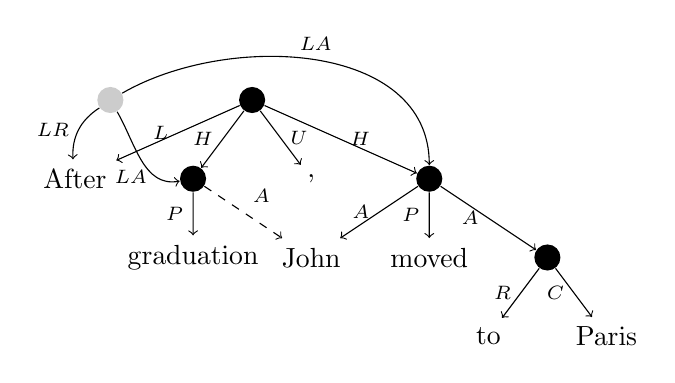
\begin{tikzpicture}[level distance=10mm, ->]
    \node (ROOT) [fill=black, circle] {}
      child {node (After) {After} edge from parent node[left] {\scriptsize $L$}}
      child {node (graduation) [fill=black, circle] {}
      {
        child {node {graduation} edge from parent node[left] {\scriptsize $P$}}
      } edge from parent node[left] {\scriptsize $H$} }
      child {node {,} edge from parent node[right] {\scriptsize $U$}}
      child {node (moved) [fill=black, circle] {}
      {
        child {node (John) {John} edge from parent node[left] {\scriptsize $A$}}
        child {node {moved} edge from parent node[left] {\scriptsize $P$}}
        child {node [fill=black, circle] {}
        {
          child {node {to} edge from parent node[left] {\scriptsize $R$}}
          child {node {Paris} edge from parent node[left] {\scriptsize $C$}}
        } edge from parent node[left] {\scriptsize $A$} }
      } edge from parent node[right] {\scriptsize $H$} }
      ;
    \draw[dashed,->] (graduation) to node [auto] {\scriptsize $A$} (John);
    \node (LKG) at (-1.8,0) [fill=black!20, circle] {};
          \draw[bend right] (LKG) to node [auto, left] {\scriptsize $LR$} (After);
          \draw (LKG) to[out=-60, in=190] node [below] {\scriptsize $LA\quad$} (graduation);
          \draw (LKG) to[out=30, in=90] node [above] {\scriptsize $LA$} (moved);
  \end{tikzpicture}
  \caption{UCCA example with linkage.}
  \label{fig:example_linkage}
\end{figure}

\paragraph{Implicit units.}

UCCA graphs may contain implicit units with no correspondent in the text.
\figref{fig:example_implicit} shows the annotation for the sentence
``A similar technique is almost impossible to apply to other crops, such as cotton, soybeans and rice.''.
The sentence was used by \newcite{oepen2015semeval} to compare between different semantic
dependency schemes.
It includes a single scene, whose main relation is ``apply'', a secondary relation ``almost impossible'', as well as two complex arguments: ``a similar technique'' and the coordinated argument ``such as cotton, soybeans, and rice.''
In addition, the scene includes an implicit argument, which represents the agent of the
``apply'' relation.

\begin{figure*}[h]
  \centering
  \scalebox{.6}{
  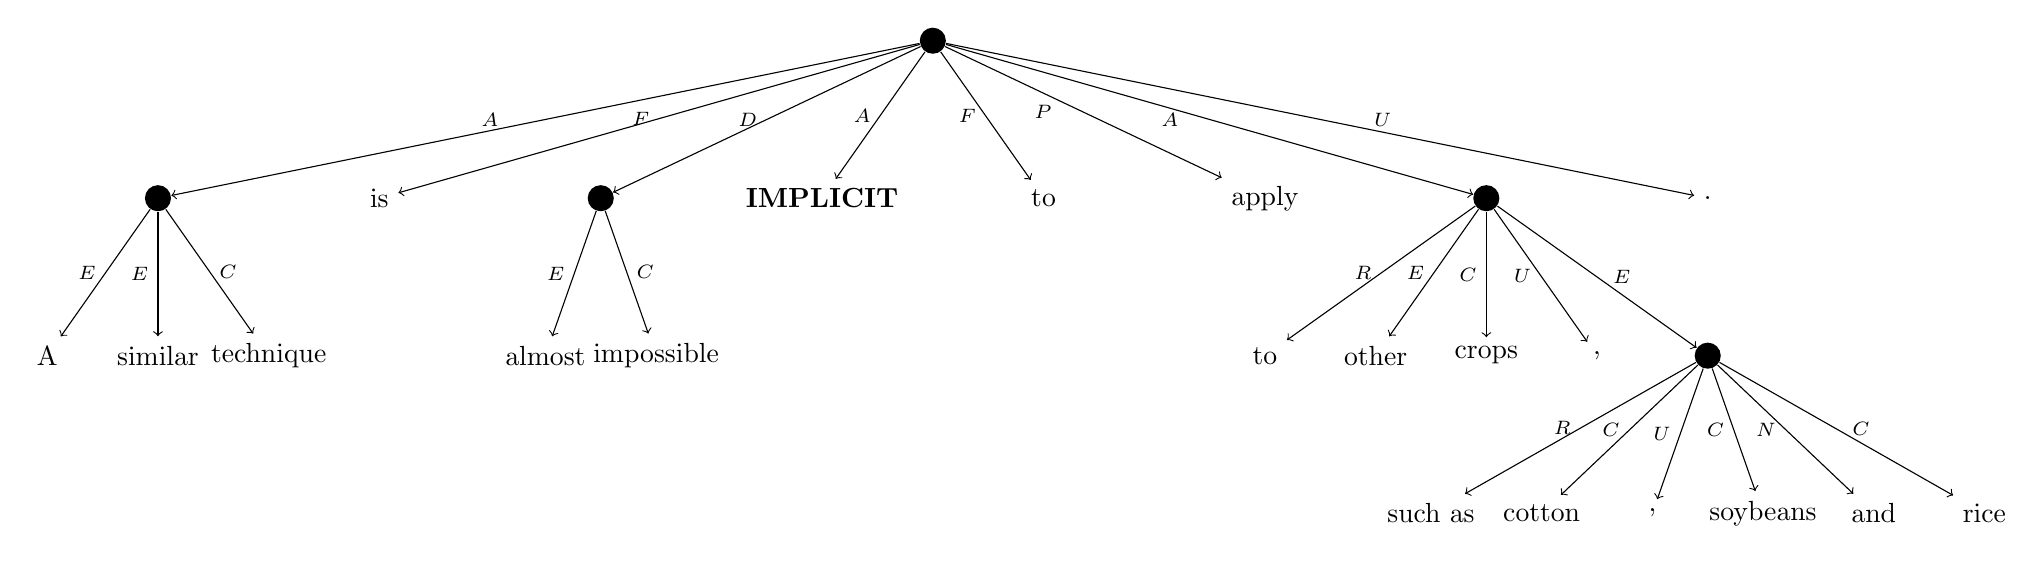
\begin{tikzpicture}[level distance=20mm, ->,
  level 1/.style={sibling distance=8em},
  level 2/.style={sibling distance=4em},
  level 3/.style={sibling distance=4em}]
    \node (ROOT) [fill=black, circle] {}
      child {node [fill=black, circle] {}
      {
        child {node {A} edge from parent node[left] {\scriptsize $E$}}
        child {node {similar} edge from parent node[left] {\scriptsize $E$}}
        child {node {technique} edge from parent node[right] {\scriptsize $C$}}
      } edge from parent node[left] {\scriptsize $A\quad$ \hspace{1mm} } }
      child {node {is} edge from parent node[left] {\scriptsize $F$}}
      child {node [fill=black, circle] {}
      {
        child {node {almost} edge from parent node[left] {\scriptsize $E$}}
        child {node {impossible} edge from parent node[right] {\scriptsize $C$}}
      } edge from parent node[left] {\scriptsize $D$} }
      child {node {\textbf{IMPLICIT}} edge from parent node[left] {\scriptsize $A$}}
      child {node {to} edge from parent node[left] {\scriptsize $F$}}
      child {node {apply} edge from parent node[left] {\scriptsize $P\quad$}}
      child {node [fill=black, circle] {}
      {
        child {node {to} edge from parent node[left] {\scriptsize $R$}}
        child {node {other} edge from parent node[left] {\scriptsize $E$}}
        child {node {crops} edge from parent node[left] {\scriptsize $C$}}
        child {node {,} edge from parent node[left] {\scriptsize $U$}}
        child {node [fill=black, circle] {}
        {
          child {node {such as} edge from parent node[left] {\scriptsize $R$}}
          child {node {cotton} edge from parent node[left] {\scriptsize $C$}}
          child {node {,} edge from parent node[left] {\scriptsize $U$}}
          child {node {soybeans} edge from parent node[left] {\scriptsize $C$}}
          child {node {and} edge from parent node[left] {\scriptsize $N$}}
          child {node {rice} edge from parent node[right] {\scriptsize $\; C$}}
        } edge from parent node[right] {\scriptsize $\; E$ \hspace{1mm} } }
      } edge from parent node[left] {\scriptsize $A\;$ \hspace{1mm} } }
      child {node {.} edge from parent node[right] {\scriptsize $\quad \quad U$}}
      ;
  \end{tikzpicture}
  }
  \caption{UCCA example with an implicit unit.}
  \label{fig:example_implicit}
\end{figure*}

The parsing of these units is deferred to future work, as it is likely to require different methods
than those explored in this paper \cite{roth2015inducing}.

\section{Hyperparameter Values}
\label{appendix:hyperparameters}

\tabref{table:hyperparameters} lists the hyperparameter values we found
for the different classifiers by tuning on the development set.
Note that learning rate decay is multiplicative and is applied at each epoch.
Mini-batch size is in number of transitions,
but a mini-batch must contain only whole sentences.

\begin{table}[h]
\centering
\scalebox{.9}{
\begin{tabular}{l|ccc}
& Sparse & MLP & BiLSTM \\
\hline
\multicolumn{4}{l}{\footnotesize Embedding dimensions} \\
external word & & 100 & 100 \\
word & & 200 & 200 \\
POS tag & & 20 & 20 \\
syntactic dep. & & 10 & 10 \\
edge label & & 20 & 20 \\
punctuation & & 1 & 1 \\
gap & & 3 & 3 \\
action & & 3 & 3 \\
\hline
\multicolumn{4}{l}{\footnotesize Other parameters} \\
training epochs & 19 & 28 & 59 \\
$\textsc{MinUpdate}$ & 5 \\
initial learning rate & 1 & 1 & 1 \\
learning rate decay & 0.1 & 1 & 1 \\
MLP \#layers & & 2 & 2 \\
MLP layer dim. & & 100 & 50 \\
LSTM \#layers & & & 2 \\
LSTM layer dim. & & & 500 \\
word dropout & & 0.2 & 0.2 \\
dropout & & 0.4 & 0.4 \\
weight decay & & $10^{-5}$ & $10^{-5}$ \\
mini-batch size & & 100 & 100
\end{tabular}
}
\caption{Hyperparameters used for the different classifiers.}
\label{table:hyperparameters}
\end{table}

\section{Bilexical Graph Conversion}
\label{appendix:conversion}

Here we describe the algorithms used in the conversion referred to in \secref{sec:exp_setup}.

\paragraph{Notation.}
Let $L$ be the set of possible edge labels.
A UCCA graph over a sequence of tokens $w_1, \ldots, w_n$ is a directed acyclic graph
$G=(V,E, \ell)$, where $\ell:E\to L$ maps edges to labels.
For each token $w_i$ there exists a leaf (\emph{terminal}) $t_i \in V$.
A bilexical (dependency) graph over the same text consists of a set $A$ of
labeled dependency arcs $(t^\prime,l,t)$
between the terminals of $G$, where $t^\prime$ is the head, $t$ is the dependent and $l$ is
the edge label.

\paragraph{Conversion to bilexical graphs.}
Let $G=(V,E,\ell)$ be a UCCA graph with labels $\ell:E\rightarrow L$.
The conversion to a bilexical graph requires calculating the set $A$.
All non-terminals in $G$ are removed.

We define a linear order over possible edge labels $L$ (see \figref{fig:priority}).
For each node $u \in V$, denote by $h(u)$ its child with the highest-priority edge label.
Let $h^*(u)$ be the terminal reached by recursively applying $h(\cdot)$ over $u$.
For each terminal $t$, we define
\[
N(t) = \{(u,v)\in E \;|\; t=h^*(v) \wedge t \neq h^*(u) \}
\]
For each edge $(u,v)\in N(t)$, we add $h^*(u)$ as a head of $t$ in $A$,
with the label $\ell(u,v)$.
This procedure is given in Algorithm~\ref{alg:to_bilexical}.

\begin{algorithm}[ht]
 \KwData{UCCA graph ${G}=(V,E,\ell)$}
 \KwResult{set $A$ of labeled bilexical arcs}
 $A \leftarrow \emptyset$\;
 \ForEach{$t \in \mathrm{Terminals}(V)$} {
  \ForEach{$(u,v)\in N(t)$} {
   $A \leftarrow A \cup \{(h^*(u), \ell(u, v), t)\}$\;
  }
 }
 \caption{Conversion to bilexical graphs.}
 \label{alg:to_bilexical}
\end{algorithm}

Note that this conversion procedure
is simpler than the head percolation procedure used for converting syntactic constituency
trees to dependency trees \cite{Coll:97},
since $h(u)$ (similar to $u$'s head-containing child)
depends only on $\ell(u,h(u))$ and not on the sub-tree spanned by $u$,
because edge labels in UCCA directly express the role of the child in the parent unit, and
are thus sufficient for determining which of $u$'s children contains the head node.

\paragraph{Conversion from bilexical graphs.}
The inverse conversion introduces non-terminal nodes back into the graph.
As the distinction between low- and high-attaching nodes is lost in the
conversion, we assume that attachments are always
low-attaching.
Let $A$ be a the labeled arc set of a bilexical graph.
Iterating over the terminals in topological order according to $A$,
we add its members as terminals to graph
and create a pre-terminal parent $u_t$ for each terminal $t$,
with an edge labeled as \textit{Terminal} between them.
The parents of the pre-terminals are determined by the terminal's parent in the bilexical
graph: if $t^\prime$ is a head of $t$ in $A$, then $u_{t^\prime}$ will be a parent of $u_t$.
We add an intermediate node in between if $t$ has any dependents in $A$,
to allow adding their pre-terminals as children later.
Edge labels for the intermediate edges are determined by a rule-based function, denoted by
$\mathrm{Label}(t)$.
This procedure is given in Algorithm~\ref{alg:from_bilexical}.

\begin{algorithm}[ht]
 \KwData{list $T$ of terminals, set $A$ of labeled bilexical arcs}
 \KwResult{UCCA graph $G=(V,E,\ell)$}
 \SetKwFunction{Label}{Label}{}{}
 $V \leftarrow \emptyset$\;
 $E \leftarrow \emptyset$\;
 \ForEach{$t \in \mathrm{TopologicalSort}(T, A)$} {
  $u_t \leftarrow \mathrm{Node()}$\;
  $V \leftarrow V \cup \{u_t, t\}$\;
  $E \leftarrow E \cup \{(u_t, t)\}$\;
  $\ell(u_t,t)\leftarrow\mathit{Terminal}$\;
  \ForEach{$t^\prime\in T,l\in L$} {
   \If{$(t^\prime,l,t)\in A$} {
    \eIf{$\exists t^{\prime\prime}\in T,l^\prime\in L : (t,l^\prime,t^{\prime\prime}) \in A$} {
     $u \leftarrow \mathrm{Node()}$\;
     $V \leftarrow V \cup \{u\}$\;
     $E \leftarrow E \cup \{(u, u_t)\}$\;
     $\ell(u, u_t) \leftarrow \Label(t)$\;
    } {
     $u \leftarrow u_t$\;
    }
    $E \leftarrow E \cup \{(u_{t^\prime}, u)\}$\;
    $\ell(u_{t^\prime}, u) \leftarrow l$\;
    }
  }
 }
 
  \SetKwProg{func}{Function}{}{}
  
  \func{\Label}{
  \KwData{node $t \in T$}
  \KwResult{label $l\in L$}

   \uIf{$\mathrm{IsPunctuation}(t)$}{
    \Return \textit{Punctuation}\;
   }
   \uElseIf{$\exists t^\prime \in T : (t,\textit{ParallelScene},t^\prime)\in A$}{
    \Return \textit{ParallelScene}\;
   }
   \uElseIf{$\exists t^\prime \in T : (t,\textit{Participant},t^\prime)\in A$}{
    \Return \textit{Process}\;
   }
   \uElse{
    \Return \textit{Center}\;
   }
  }
 \caption{Conversion from bilexical graphs.}
 \label{alg:from_bilexical}
\end{algorithm}

\begin{figure}[ht]
\begin{enumerate}
\itemsep0em
\item $C$ (Center)
\item $N$ (Connector)
\item $H$ (ParallelScene)
\item $P$ (Process)
\item $S$ (State)
\item $A$ (Participant)
\item $D$ (Adverbial)
\item $T$ (Time)
\item $E$ (Elaborator)
\item $R$ (Relator)
\item $F$ (Function)
\item $L$ (Linker)
\item $LR$ (LinkRelation)
\item $LA$ (LinkArgument)
\item $G$ (Ground)
\item $\mathit{Terminal}$ (Terminal)
\item $U$ (Punctuation)
\end{enumerate}
\caption{Priority order of edge labels used by $h(u)$.}
\label{fig:priority}
\end{figure}

\clearpage
\bibliography{references}
\bibliographystyle{acl_natbib}

\end{document}
